%% Default preamble BEGIN
\documentclass[oneside]{memoir}

\usepackage{./custom}

%% Title Page
\title{\centering
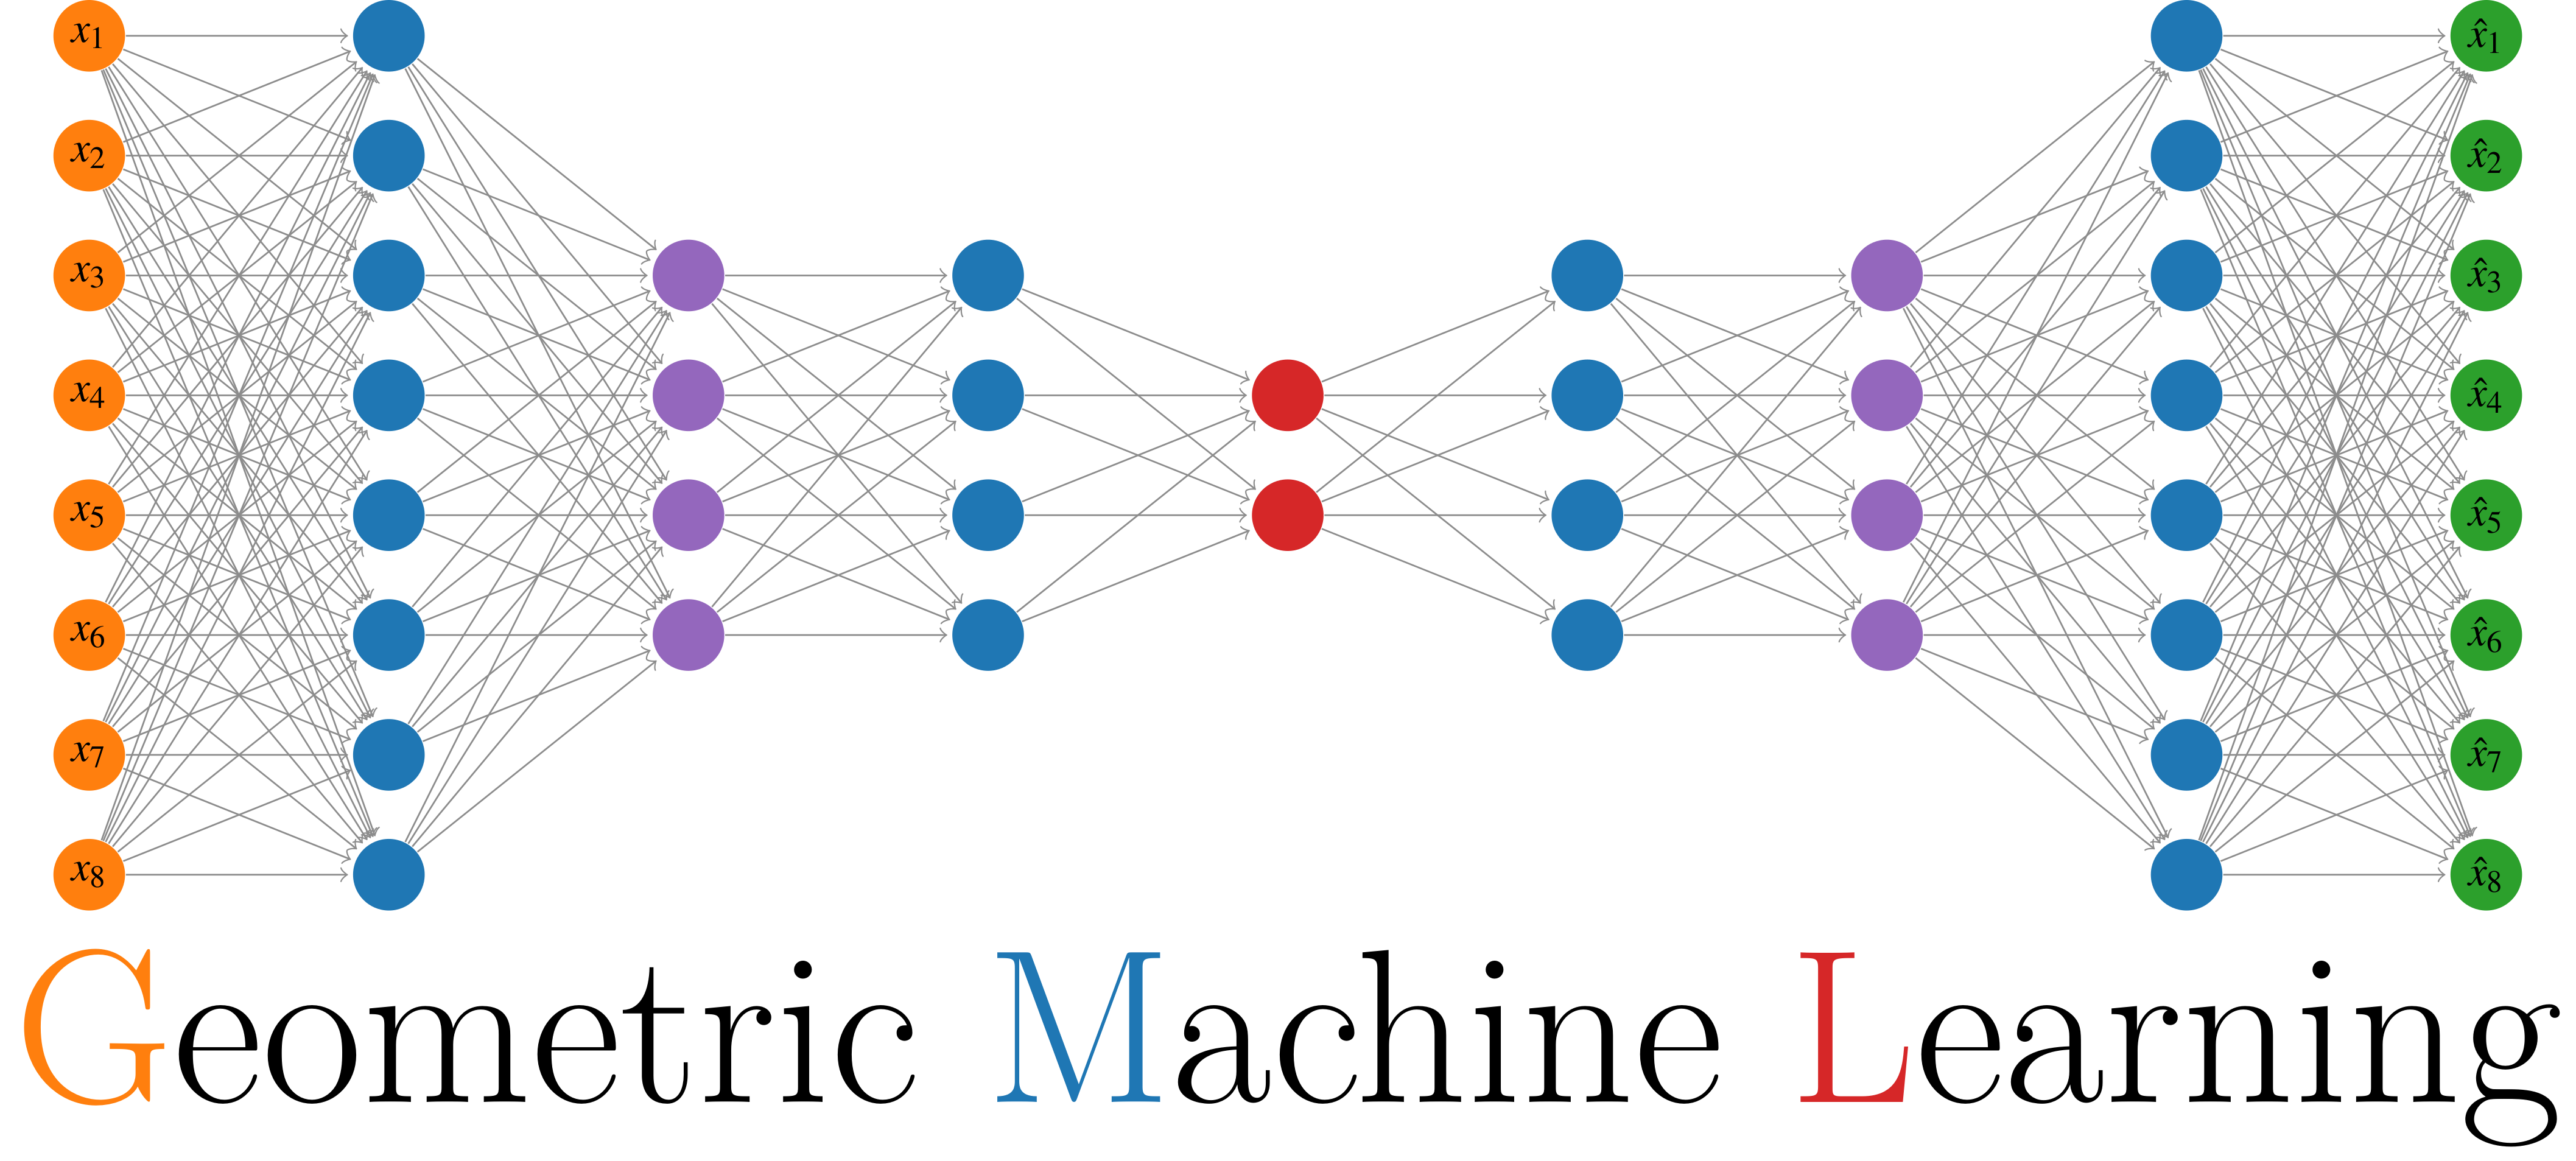
\includegraphics[width=.8\textwidth]{assets/logo_without_jl.png}
}
\author{Benedikt Brantner}

\makeatletter       
\def\@maketitle{
\raggedright

\includegraphics[height = 13mm]{assets/logo_ipp.jpg}\hfill
\includegraphics[height = 13mm]{assets/logo_tum.pdf}\\[18ex]
\begin{center}
{\Huge \bfseries \sffamily \@title }\\[4ex] 
{\Large  \@author}\\[4ex] 
\@date\\[8ex]
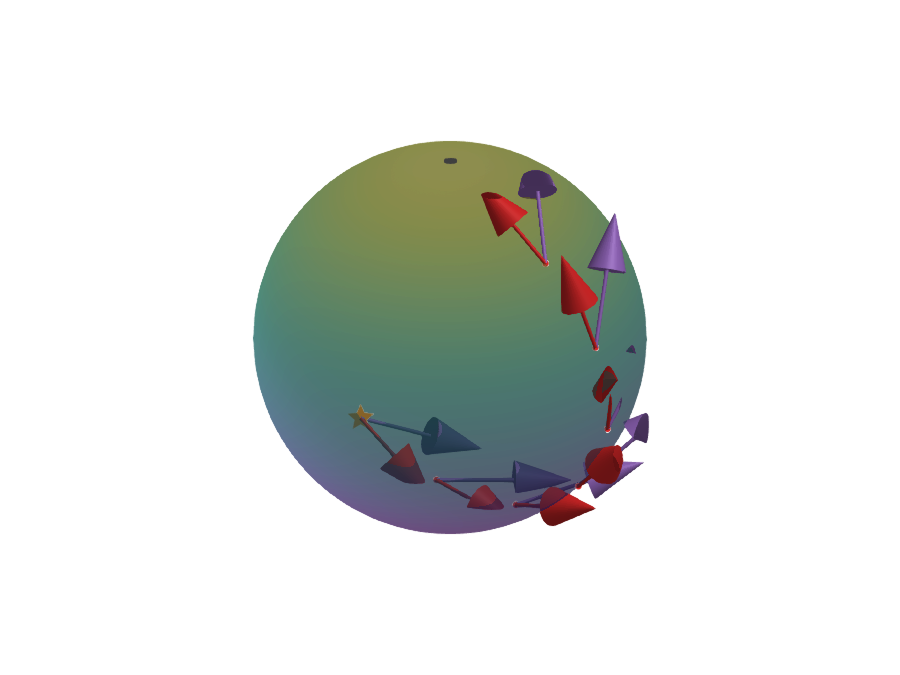
\includegraphics[height = 65mm]{parallel_transport_naked.png}
\end{center}}
\aliaspagestyle{title}{empty} % suppress the page number after \maketitle
\makeatother
\hyphenation{wiss-en-schaft-lich-en}

%% TOC settings
% -- TOC depth
%   value: [part, chapter, section, subsection,
%           subsubsection, paragraph, subparagraph]
\settocdepth{section}  % show "part+chapter+section" in TOC
% -- TOC spacing
%   ref: https://tex.stackexchange.com/questions/60317/toc-spacing-in-memoir
%   doc: memoir/memman.pdf
%       - Figure 9.2: Layout of a ToC
%       - Table 9.3: Value of K in macros for styling entries
\makeatletter
% {part} to {chapter}
\setlength{\cftbeforepartskip}{1.5em \@plus \p@}
% {chapter} to {chapter}
\setlength{\cftbeforechapterskip}{0.0em \@plus \p@}
% Part num to chapter title spacing
\setlength{\cftpartnumwidth}{2.5em \@plus \p@}
% Chapter num to chapter title spacing
\setlength{\cftchapternumwidth}{2.5em \@plus \p@}
% indent before section number
\setlength{\cftsectionindent}{2.5em \@plus \p@}
% Section num to section title spacing
\setlength{\cftsectionnumwidth}{4.0em \@plus \p@}
\makeatother

%% Main document begin
\begin{document}

\frontmatter
\maketitle
\clearpage
\setcounter{page}{1}

\thispagestyle{empty}
% \includegraphics[height=0.1\textwidth]{figures/logos/rohan/faculty.pdf} 
\hfill

\includegraphics[height=0.1\textwidth]{assets/logo_tum.pdf}
\vspace*{0.5cm}

\begin{center}
	{\Large Technische Universit\"at M\"unchen}
\end{center}
\vspace*{0.5cm}

\begin{center}
	{\Large TUM School of Computation, Information and Technology}
\end{center}
\vspace*{0.5cm}


\begin{center}
	{
		\LARGE\textbf{\getTitle - }\par
		\vspace{0.3cm}
		\large \textbf{\getSubTitle}\par
	}
\end{center}
\vspace*{0.5cm}

\begin{center}
	{\Large \textbf{\getAuthor}}
\end{center}
\vspace*{1.0cm}

\vfill
{\setlength{\parindent}{0cm} Vollst\"andiger Abdruck der von der TUM School of Computation, Infromation and Technology der Technischen Universit\"at M\"unchen zur Erlangung des akademischen Grades eines}
%\vspace*{-0.3cm}
\begin{center}
	{Doktors der Naturwissenschaften}
\end{center}
%\vspace*{-0.3cm}
{genehmigten Dissertation.}
\vspace*{1cm}
\begin{table}[h]
	\centering
	\begin{tabular}{ll}
		{Vorsitz:}  & {\;\;\; \getChairman} \\
		& \\
		{Pr\"ufer der Dissertation:} & \\
		& {1. \getSupervisor} \\
		& \\	
		& {2. \getExaminer} \\
		& \\
		& {3. \getSecondExaminer} \\
	\end{tabular}
\end{table}
\vspace*{1cm}

{\setlength{\parindent}{0cm} Die Dissertation wurde am \getSubmissionDate\ bei
	der Technischen Universit\"at M\"unchen eingereicht und durch die
	TUM School of Computation, Information and Technology
	am \getAcceptanceDate\ angenommen.}

\pagestyle{empty}

%% preamble END
